\section{Phenix Superpose PDBs protocol}
\label{app:superposePdbsProtocol}%a150
Protocol designed to refine in real space an atomic structure into a map in \scipion by using \iii{phenix.superpose\_pdbs} program \citep{zwartUrl}. Integrated in the $Phenix$ software suite (\url{https://www.phenix-online.org/}), \phenix protocol \scommand{phenix - superpose pdbs} allows to compare visually the geometry of two atomic structures by overlapping them. Root mean square deviation (RMSD) between fixed and moving structures is computed before and after the superposition. 

\begin{itemize}
 \item Requirements to run this protocol and visualize results:
    \begin{itemize}
        \item \scipion plugin: \ttt{scipion-em-phenix}
        \item PHENIX software suite (version 1.13-2998)
        \item \scipion plugin: \ttt{scipion-em-chimera}
    \end{itemize}
 \item \scipion menu:\\
  \ttt{Protocols SPA -> Tools -> Calculators} (\ffigure{fig:app_protocol_superpose_pdbs_1} (A))\\
  
 \item Protocol form parameters (\ffigure{fig:app_protocol_superpose_pdbs_1} (B)):\\
 
 \begin{figure}[H]
     \centering 
     \captionsetup{width=.7\linewidth} 
     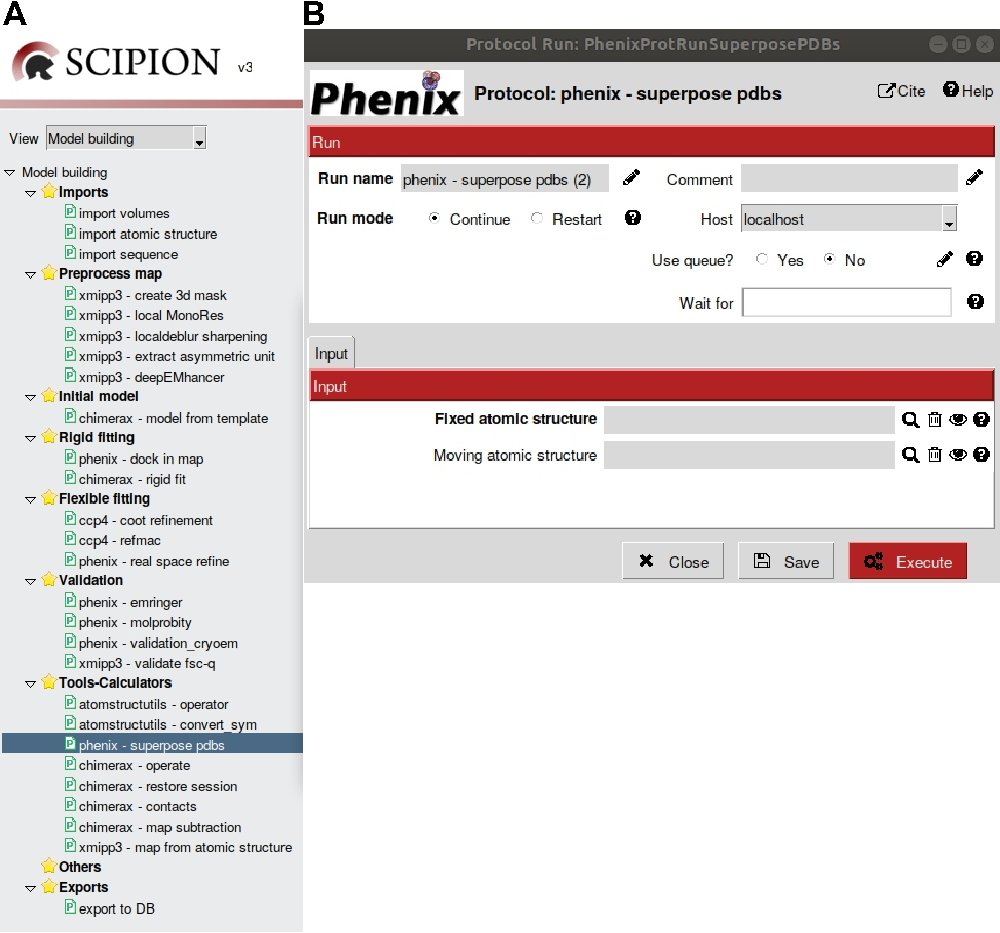
\includegraphics[width=0.90\textwidth]{Images_appendix/Fig153.pdf}
     \caption{Protocol \scommand{phenix - superpose pdbs}. A: Protocol location in \scipion menu. B: Protocol form.}
     \label{fig:app_protocol_superpose_pdbs_1}
    \end{figure}
    
   \begin{itemize}
    \item \ttt{Fixed atomic structure}: Fixed PDBx/mmCIF, previously downloaded or generated in \scipion, to which the moving one will be aligned. 
    \item \ttt{Moving atomic structure}: PDBx/mmCIF, previously downloaded or generated in \scipion, that will be aligned to the fixed one.
   \end{itemize}
 
 \item Protocol execution:\\
 Adding specific sequence label is recommended in \ttt{Run name} section, at the form top. To add the label, open the protocol form, press the pencil symbol at the right side of \ttt{Run name} box, complete the label in the new opened window, press OK, and finally close the protocol. This label will be shown in the output summary content (see below). If you want to run again this protocol, do not forget to set to \ttt{Restart} the \ttt{Run mode}.\\
  Press the \ttt{Execute} red button at the form bottom.\\
  
 \item Visualization of protocol results:\\
 
 After executing the protocol, press \ttt{Analyze Results} and and \chimera graphics window will be opened by default. Atomic structures and volumes are referred to the origin of coordinates in \chimera. To show the relative position of atomic structure and electron density volume, the three coordinate axes are represented; X axis (red), Y axis (yellow), and Z axis (blue) (\ffigure{fig:app_protocol_volume_3}).\\
    
 \item Summary content:\\
 
  \ttt{SUMMARY} box:\\RMSD between fixed and moving atoms (start and final values).
\end{itemize}

